\section{Methodology And Project Schedule}
\subsection{Project Methodology}
This project is fundamentally a design project and so the design will heavily depend on the system functional and non-functional requirements as defined in table \ref{tab:FRandNFR}. These requirements will be verified through experimental analysis using both the mechanical and electrical engineering laboratories, and the Griffith footbridge. The experimental verification methods include integration testing, environmental testing and field testing. The testing methods required to validate each requirement is also defined in table \ref{tab:FRandNFR}. Additional to these requirements, closed loop testing will provide experimental analysis to verify that the accelerometers, temperature sensors, ADC conversion, packet transmission and retrieval meet the design requirements of the system. Testing will also be conducted on the designed enclosure to ensure the system is sufficiently weather proofed against heat and rain.  

\subsection{Tasks and Schedule}
Figure \ref{fig:GanttChart} displays the rough timeline for the completion of this project. This timeline also includes professional practice deadlines. 

\begin{figure}[h!]
\center
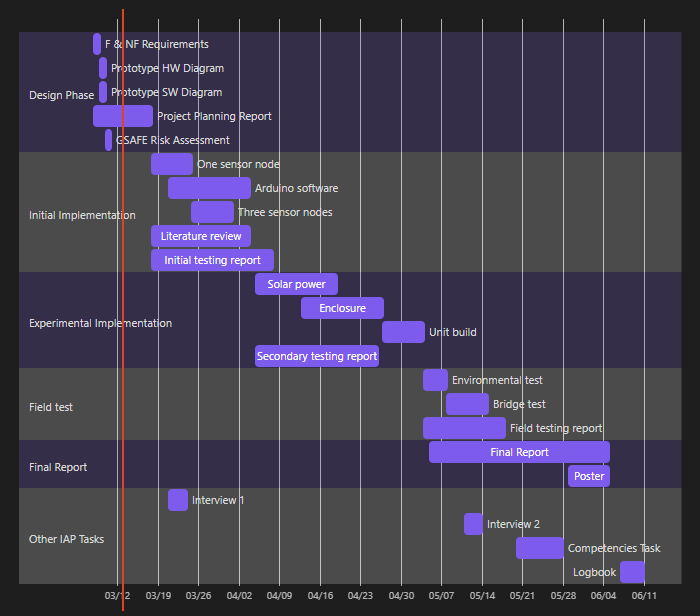
\includegraphics[scale=0.8]{Images/Gantt-Chart.png}
\caption{Project Timeline Gantt Chart}
\label{fig:GanttChart}
\end{figure}

\subsection{Resources}




